\documentclass[10pt]{article}
\usepackage[T1]{fontenc} % Use T1 font encoding
\usepackage[utf8]{inputenc} % Ensure UTF-8 encoding
\usepackage[polish, provide=*]{babel}
\usepackage{amsmath}
\usepackage{graphicx}
\usepackage{booktabs}
\usepackage{float}
\usepackage[margin=2.5cm]{geometry}
\usepackage{siunitx}
\usepackage{titlesec}
\titlespacing*{\subsection}{0pt}{*0.5}{*0.5} % Adjusts spacing before and after subsections
\usepackage{caption}
\usepackage{lmodern}
\usepackage{placeins} % For FloatBarrier
\usepackage{hyperref} % For hyperlinks in the document
\usepackage{threeparttable} % For better table handling
\usepackage{longtable} % For tables spanning multiple pages
\usepackage{fancyhdr} % For headers and footers
\usepackage{array} % For better table formatting
\usepackage{xcolor} % For colors

\title{Diody}
\date{}

\begin{document}

% --------------------------- STRONA TYTUŁOWA --------------------------
\thispagestyle{empty} % Remove page number from title page

\begin{center}
    {\Large\textbf{UNIWERSYTET RADOMSKI}} \\
    \textit{im. Kazimierza Pułaskiego w Radomiu} \\
    \vspace{0.3cm}
    {\large\textbf{LABORATORIUM PODSTAW ELEKTRONIKI}} \\
\end{center}

\vspace{1.5cm}

% Main information box
\begin{center}
\fbox{\begin{minipage}{0.9\textwidth}
\centering
\vspace{0.5cm}
{\Large\textbf{SPRAWOZDANIE Z ĆWICZENIA}} \\
\vspace{0.8cm}
{\LARGE\textbf{Diody}} \\
\vspace{0.5cm}
\end{minipage}}
\end{center}

\vspace{1.5cm}

% Information table
\begin{center}
\begin{tabular}{|>{\bfseries}p{4cm}|p{6cm}|}
\hline
Wydział: & WTEiI \\
\hline
Kierunek: & Informatyka \\
\hline
Rok Akademicki: & 2024/2025 \\
\hline
Semestr: & II \\
\hline
Grupa: & 3 \\
\hline
Zespół: & 2 \\
\hline
Wykonujący: & Jakub Oleszczuk \\
& Mateusz Ofiara \\
& Mikołaj Majewski \\
& Onolbataar Tumentur \\
\hline
Ocena: &  \\
\hline
\end{tabular}
\end{center}

\vspace{2cm}

% --------------------------- TREŚĆ SPRAWOZDANIA --------------------------
\subsection*{Cel ćwiczenia}
Celem ćwiczenia jest zapoznanie się z charakterystyką prądowo-napięciową diod półprzewodnikowych, 
w tym diody Germanowej, Krzemowej, LED oraz Zenera. 
Ćwiczenie ma na celu zrozumienie działania diod w różnych kierunkach przewodzenia i zaporowym, a także umiejętność analizy wyników pomiarów.
\subsection*{Wprowadzenie teoretyczne}
Dioda półprzewodnikowa to element elektroniczny, który pozwala na przepływ prądu w jednym kierunku, 
a blokuje go w kierunku przeciwnym. Działanie diody opiera się na zjawisku zwanemu złączem p-n, 
które powstaje w wyniku połączenia dwóch rodzajów półprzewodników: typu p (z nadmiarem dziur) i typu n (z nadmiarem elektronów). 
W momencie przyłożenia napięcia w kierunku przewodzenia, złącze p-n staje się przewodzące, co pozwala na przepływ prądu. 
W przeciwnym przypadku, gdy napięcie jest przyłożone w kierunku zaporowym, złącze to blokuje przepływ prądu.
\clearpage
\subsection*{Wyniki pomiarów}
\begin{table}[!ht]
    \centering
    \caption{Wyniki pomiarów charakterystyki prądowo-napięciowej diody Germanowej w kierunku przewodzenia}
    \begin{tabular}{|l|l|l|l|l|l|l|l|l|}
    \hline
        I[ µA] & 10 & 20 & 50 & 100 & 200 & 500 & 1000 & 5000 \\ \hline
        U [V] & 0,009 & 0,016 & 0,034 & 0,052 & 0,075 & 0,113 & 0,147 & 0,238 \\ \hline
    \end{tabular}
\end{table}
\begin{table}[!ht]
    \centering
    \caption{Wyniki pomiarów charakterystyki prądowo-napięciowej diody Germanowej w kierunku zaporowym}
    \begin{tabular}{|l|l|l|l|l|l|}
    \hline
        U [V] & 5 & 10 & 15 & 20 & 30 \\ \hline
        I[ µA] & 93,2 & 213,1 & 364 & 519,7 & 807 \\ \hline
    \end{tabular}
\end{table}
\begin{table}[!ht]
    \centering
    \caption{Wyniki pomiarów charakterystyki prądowo-napięciowej diody Krzemowej w kierunku przewodzenia}
    \begin{tabular}{|l|l|l|l|l|l|l|l|l|}
    \hline
        I[uA] & 10 & 20 & 50 & 100 & 200 & 500 & 1000 & 5000 \\ \hline
        U [V] & 0,393 & 0,416 & 0,449 & 0,478 & 0,503 & 0,546 & 0,578 & 0,653 \\ \hline
    \end{tabular}
\end{table}
\begin{table}[!ht]
    \centering
    \caption{Wyniki pomiarów charakterystyki prądowo-napięciowej diody LED w kierunku przewodzenia}
    \begin{tabular}{|l|l|l|l|l|l|l|l|l|}
    \hline
        I[ µA] & 10 & 20 & 50 & 100 & 200 & 500 & 1000 & 5000 \\ \hline
        U [V] & 1,41 & 1,447 & 1,435 & 1,581 & 1,557 & 1,608 & 1,642 & 1,793 \\ \hline
    \end{tabular}
\end{table}
\begin{table}[!ht]
    \centering
    \caption{Wyniki pomiarów charakterystyki prądowo-napięciowej diody Zenera w kierunku przewodzenia}
    \begin{tabular}{|l|l|l|l|l|l|l|l|l|}
    \hline
        I[ µA] & 10 & 20 & 50 & 100 & 200 & 500 & 1000 & 5000 \\ \hline
        U [V] & 5,168 & 5,535 & 5,95 & 6,21 & 6,445 & 6,61 & 6,65 & 6,68 \\ \hline
    \end{tabular}
\end{table}
\begin{table}[!ht]
    \centering
    \caption{Wyniki pomiarów charakterystyki prądowo-napięciowej diody Zenera w kierunku zaporowym}
    \begin{tabular}{|l|l|l|l|l|l|l|l|l|}
    \hline
        I[ µA] & 10 & 20 & 50 & 100 & 200 & 500 & 1000 & 5000 \\ \hline
        U [V] & 0,433 & 0,479 & 0,518 & 0,543 & 0,57 & 0,609 & 0,632 & 0,684 \\ \hline
    \end{tabular}
\end{table}
\clearpage
\subsection*{Charakterystyki prądowo-napięciowe}

\begin{figure}[H]
    \centering
    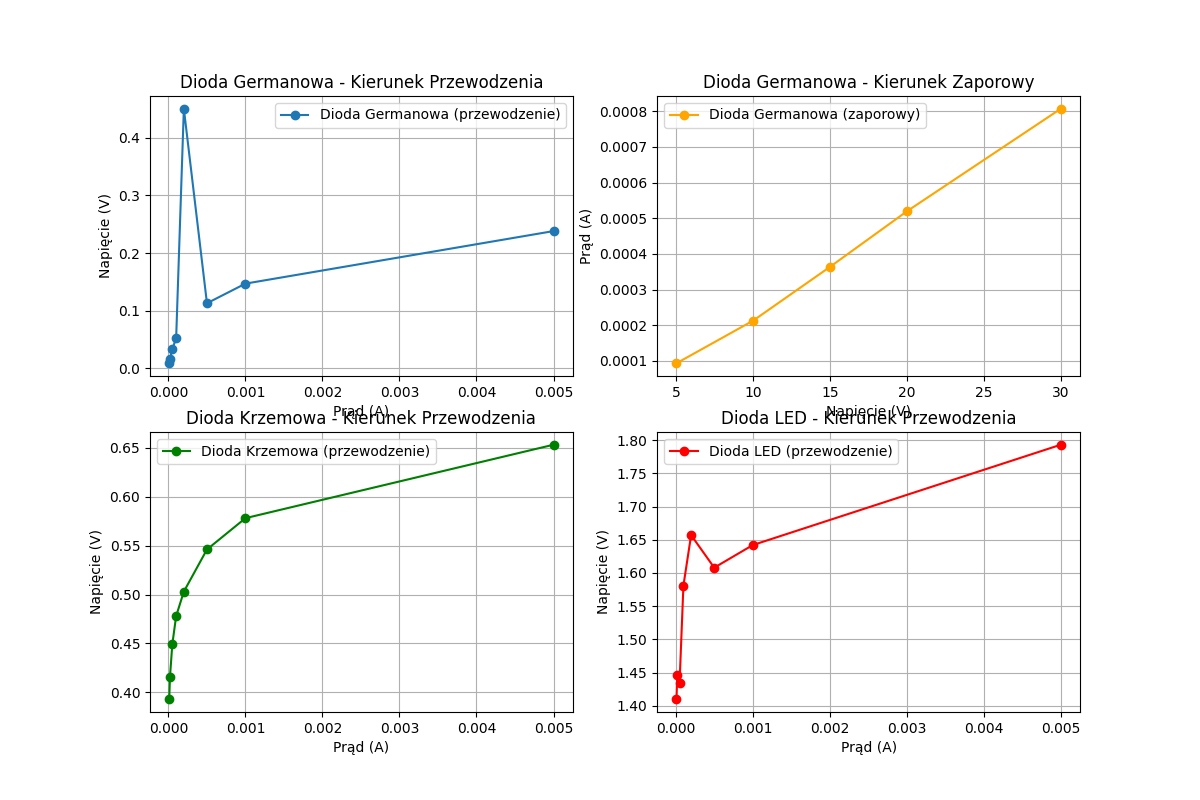
\includegraphics[width=1.0\textwidth]{Figure_1.png}
    \caption{Charakterystyki prądowo-napięciowe diod Germanowej, Krzemowej, LED}
    \label{fig:charakterystyki_przewodzenie}
\end{figure}

\begin{figure}[H]
    \centering
    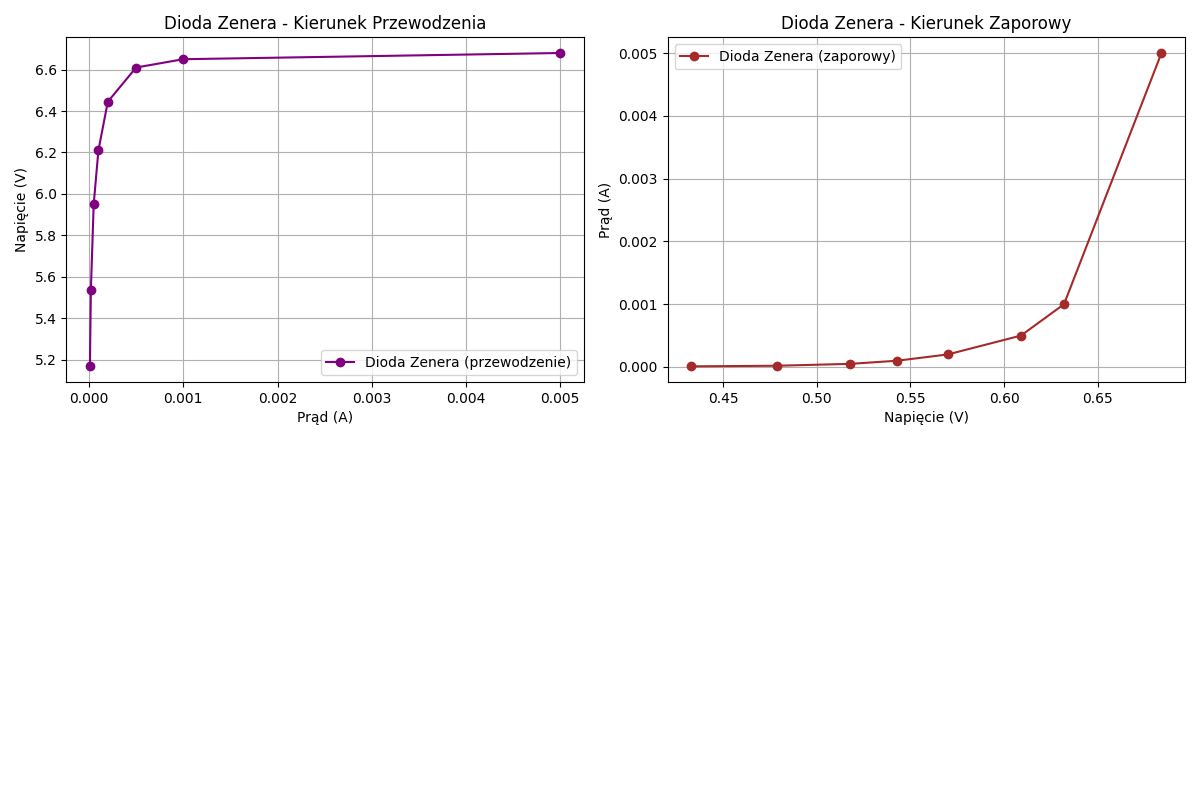
\includegraphics[width=0.9\textwidth]{Figure_2.png}
    \caption{Charakterystyki prądowo-napięciowe diody Zenera w kierunku przewodzenia i zaporowym}
    \label{fig:charakterystyki_zaporowy}
\end{figure}
\subsection*{Analiza Wyników}
Na podstawie pomiarów i wykresów przedstawionych na rysunkach \ref{fig:charakterystyki_przewodzenie} i \ref{fig:charakterystyki_zaporowy}, można zaobserwować charakterystyczne właściwości różnych typów diod półprzewodnikowych.

Dioda Germanowa charakteryzuje się niskim napięciem przewodzenia, co czyni ją odpowiednią do zastosowań w niskonapięciowych układach elektronicznych.
Dioda Krzemowa ma wyższe napięcie przewodzenia, ale jest bardziej stabilna i odporna na wysokie temperatury, co czyni ją bardziej uniwersalną w zastosowaniach elektronicznych.
Dioda LED, będąca specjalnym rodzajem diody, emituje światło podczas przewodzenia prądu, co czyni ją idealną do zastosowań w oświetleniu i sygnalizacji.
Dioda Zenera, z kolei, jest wykorzystywana głównie w obwodach stabilizacyjnych, gdzie jej charakterystyka zaporowa pozwala na utrzymanie stałego napięcia.

\subsection*{Podsumowanie}
W ćwiczeniu przeanalizowano charakterystyki prądowo-napięciowe różnych typów diod półprzewodnikowych, w tym diody Germanowej, Krzemowej, LED oraz Zenera.
Dzięki pomiarom i analizie wyników, uczestnicy ćwiczenia zyskali praktyczne umiejętności w zakresie analizy działania diod w różnych warunkach pracy.

\end{document}
